
\documentclass[12pt]{report}
\usepackage[utf8]{inputenc}

\usepackage{listings}
\usepackage{graphicx}
\usepackage{amsmath}
\usepackage{amsfonts}
\usepackage{amssymb}
\usepackage{pgfgantt}
\usepackage{amsthm}
\usepackage{fancyhdr}
\usepackage{rotating}
\usepackage[graphicx]{realboxes}
\renewcommand{\vec}{\bm}
\usepackage{dsfont}
\usepackage{xcolor}
\usepackage{sectsty}
\usepackage{tikz}
\usepackage{pgfplots}
% \usepackage[backend=biber]{biblatex}
% \addbibresource{report.bib}
\pgfplotsset{compat=newest}
\usepgfplotslibrary{patchplots}
\usetikzlibrary{calc,intersections,trees,positioning,arrows,chains,shapes.geometric,%
    decorations.pathreplacing,decorations.pathmorphing,shapes,%
    matrix,shapes.symbols, 3d}


\tikzset{
>=stealth',
  punktchain/.style={
    rectangle,
    rounded corners,
    % fill=black!10,
    draw=black, very thick,
    text width=10em,
    minimum height=3em,
    text centered,
    on chain},
  line/.style={draw, thick, <-},
  element/.style={
    tape,
    top color=white,
    bottom color=blue!50!black!60!,
    minimum width=8em,
    draw=blue!40!black!90, very thick,
    text width=10em,
    minimum height=3.5em,
    text centered,
    on chain},
  every join/.style={->, thick,shorten >=1pt},
  decoration={brace},
  tuborg/.style={decorate},
  tubnode/.style={midway, right=2pt},
  pics/carc/.style args={#1:#2:#3}{
    code={
      \draw[pic actions] (#1:#3) arc(#1:#2:#3);
    }
  }
}

% set the default code style
\lstset{
    frame=tb, % draw a frame at the top and bottom of the code block
    tabsize=4, % tab space width
    showstringspaces=false, % don't mark spaces in strings
    numbers=left, % display line numbers on the left
    basicstyle=\ttfamily,
    language=C++,
    breaklines=true,
    commentstyle=\color{gray}\ttfamily,, % comment color
    keywordstyle=\color{blue}\ttfamily,, % keyword color
    stringstyle=\color{red}\ttfamily, % string color
}

\usepackage[paper=a4paper,top=0.58in,left=1.65in, right=1.65in, bottom=1.65in]{geometry}

\definecolor{lightorange}{RGB}{251,211,168}
\definecolor{darkred}{RGB}{153,0,0}
\definecolor{darkgreen}{RGB}{0,51,25}

\title{ \includegraphics[width=\linewidth]{header.png}~
\\[0.5cm]
  \huge{Bachelor Project} \\
\textbf{\Large{Barycentric Data Visualization for Triangle Meshes}}}
\date{Spring Semester 2018}
\author{Costanza \textbf{Volpini} \\ \textcolor{gray}{costanza.volpini@usi.ch} \\ \\ Professor: Kai \textbf{Hormann} \\ Assistant: Jan \textbf{Svoboda}}

\begin{document}
\pagestyle{fancy}
\rhead{\bfseries  Costanza Volpini}
\lhead{\bfseries  Bachelor Project}
\maketitle
\newgeometry{paper=a4paper,margin=1.65in}

%%%%%%% ref: https://it.sharelatex.com/blog/2013/08/02/thesis-series-pt1.html
\chapter*{Abstract}
Abstract goes here (?)
% The power of barycentric coordinates will grant the exploration of alternative data visualization techniques.

\chapter*{Dedication}
to somebody (?)

\chapter*{Declaration}
I declare that.. (?)

\chapter*{Acknowledgements}
I want to thank... (?)

\tableofcontents
%%%%%%%
\chapter{Introduction}
\section{Barycentric coordinates}
Let us consider a triangle with top, bottom left and bottom right vertices to which we have assigned the colors red, green and blue respectively. The triangle barycentre divides each median into two parts that have a 2:1 ratio. \\
  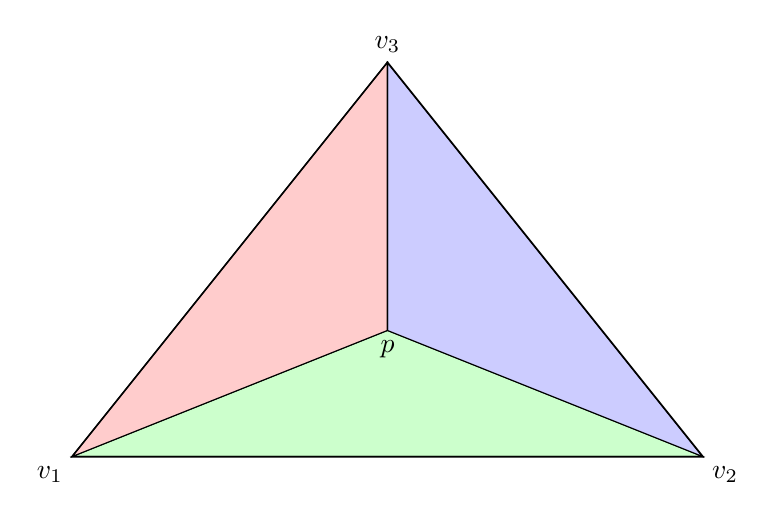
\begin{tikzpicture}
    \coordinate (L1) at (0,0);
    \coordinate (L2) at (8,0);
    \coordinate (L3) at (4,5);
    \coordinate (X) at (4,1.6);

    \draw[thick] (L1) -- coordinate[midway](md3) (L2)
                      -- coordinate[midway](md1) (L3)
                      -- coordinate[midway](md2) (L1) -- cycle;
    \filldraw[draw=black, fill=green!20] (L1) -- (X) -- (L2) -- cycle;
    \filldraw[draw=black, fill=red!20] (L1) -- (X) -- (L3) -- cycle;
    \filldraw[draw=black, fill=blue!20] (L3) -- (X) -- (L2) -- cycle;
    \draw (L1) node [below left] {$v_1$}
       -- (L2) node [below right] {$v_2$}
       -- (L3) node [above] {$v_3$}
       -- (X) node [below] {$p$};
    \end{tikzpicture}
    \\
    Let call the red area $w_1$, the blue green one $w_2$ and the blue one $w_3$. Normalazing each of them by the area of the triangle, we will get three values ($\lambda_1, \lambda_2, \lambda_3$) that are the barycentric coordinates of $p$ with respect to the triangle [$v_1, v_2, v_3$].
\\ \\ WRITE!!!!!!! introduction and all properties

\section{Linear Interpolation}
The standard linear interpolated visualisation is made passing three attributes (colors) for each vertex of a triangle. OpenGL will interpolate linearly the colors. That is possible thanks to the barycentric coordinates that will tell how much of each color is being mixed at any position.

\section{Flat Shading}

\section{Gouraud Shading}

\section{Gaussian Curvature}
\textit{Gaussian Curvature} works like a logical \texttt{AND}, it will check if there is a curvature along both directions.

\begin{figure}[h]
  \minipage[b]{.5\linewidth}
  \centering
  \scalebox{0.7}{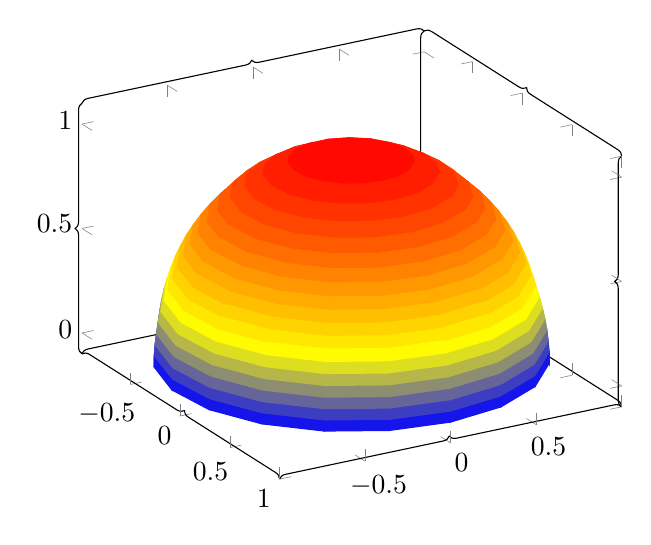
\begin{tikzpicture}
  \begin{axis}[view={60}{30}]
      \addplot3[surf,shader=flat,
          samples=20,
          domain=1:0,y domain=0:2*pi,
          z buffer=sort]
          ({sqrt(1-x^2) * cos(deg(y))},
       {sqrt( 1-x^2 ) * sin(deg(y))},
       x);
  \end{axis}
  \end{tikzpicture}}
  \caption{Positive gaussian curvature}\label{fig:positive-gaussian}
  \endminipage
  \minipage[b]{.5\linewidth}
  \centering
  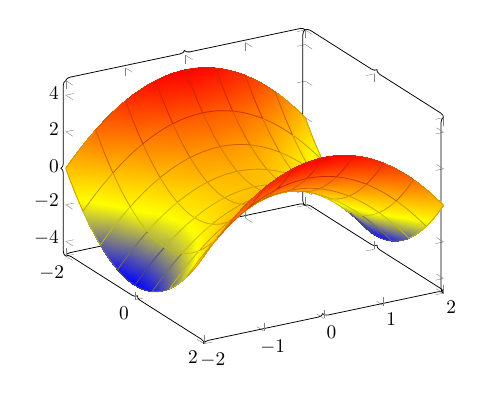
\begin{tikzpicture}[scale=0.7]
    \begin{axis}[view={60}{30}]
    \addplot3[patch,patch refines=3,
    shader=faceted interp,
    patch type=biquadratic]
    table[z expr=x^2-y^2]
    {
        x  y
        -2 -2
        2  -2
        2  2
        -2 2
        0  -2
        2  0
        0  2
        -2 0
        0  0
    };
  \end{axis}
  \end{tikzpicture}
  \endminipage
  \caption{Negative gaussian curvature}\label{fig:negative-gaussian}
\end{figure}


\chapter{GPU program}
shaders (geometry, vertex, fragment) + model view etc.
arcball/trackball

Shader program is written in \textit{GLSL}.

Vertex shader is done on every vertex (before rasterization).
Fragment shader is done on every pixel (coloring per fragment).

%%%%%%%%%
A program that runs on GPU is called \textit{shader}. Shaders are principally used to modify the representation and the behaviour of 3D objects. They are also used to create lighting effects.  Shaders can perform tasks efficiently thanks to the GPU. That guarantee faster results than CPU since GPU is designed to work in parallel.

\section{GPU pipeline}
% \\
% \\
\scalebox{0.85}{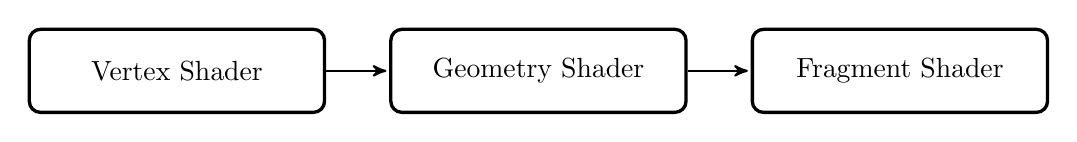
\begin{tikzpicture}
    [node distance=.8cm,
    start chain=going right,]
       \node[punktchain, join] (vs) {Vertex Shader};
       \node[punktchain, join] (gs)  {Geometry Shader};
       \node[punktchain, join] (fs)  {Fragment Shader};
\end{tikzpicture}}


\section{Vertex Shader}
The program that perform vertex operations is called \textit{vertex shader}. It receives one vertex at a time and then it passes the output to a \textit{fragment shader} or to a \textit{geometry shader}, if any.

\section{Fragment Shader}
\textit{Fragment shader} performs color computation for every visible pixel of the rasterized object. It works on a fragment at a time, but thanks to the power of GPU it can work in parallel for all vertices (\textit{vertex shader}) and fragments (\textit{fragment shader}).

\section{Geometry Shader}
\textit{Geometry shader} is used for layered rendering. It takes as input a set of vertices (single primitive, example: triangle or a point) and it transforms them before sending to the next shader stage. In this way, we can obtain different primitives.

Each time we call the function \texttt{EmitVertex()} the vector currently set to \texttt{gl\_Position} is added to the primitive. All emitted vertices are combined for the primitive and output when we call the function \texttt{EndPrimitive()}.
\\
\\
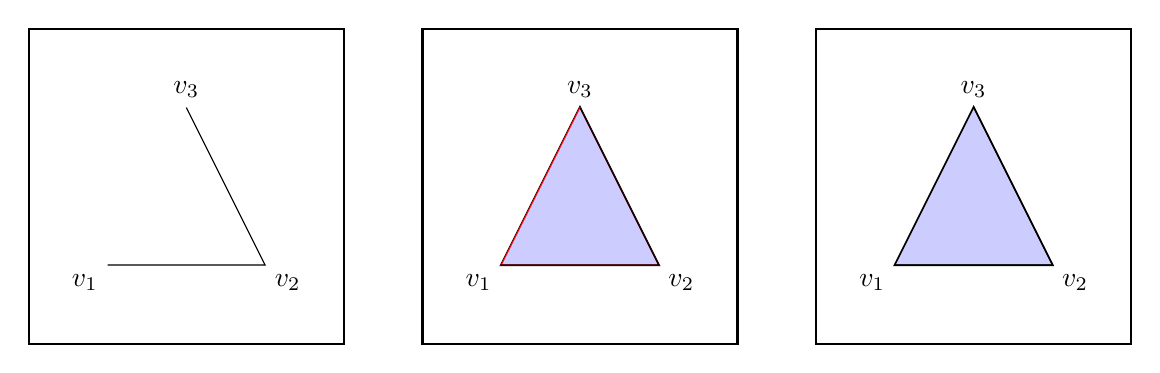
\begin{tikzpicture}
    \coordinate (L1) at (6,0);
    \coordinate (L2) at (8,0);
    \coordinate (L3) at (7,2);

    \coordinate (S1) at (5,-1);
    \coordinate (S2) at (9,-1);
    \coordinate (S3) at (5,3);
    \coordinate (S4) at (9,3);


    % \draw[thick] (L1) -- (L2)
    %                   -- (L3)
    %                   -- (L1) -- cycle;


    \draw[thick] (S1) --  (S2)
                      --  (S4)
                      --  (S3)
                      --  (S1) -- cycle;



    \coordinate (L11) at (11,0);
    \coordinate (L12) at (13,0);
    \coordinate (L13) at (12,2);

    \coordinate (S11) at (10,-1);
    \coordinate (S12) at (14,-1);
    \coordinate (S13) at (10,3);
    \coordinate (S14) at (14,3);


    \draw[thick] (L11) -- (L12)
                      -- (L13)
                      -- (L11) -- cycle;

    \draw[thick] (S11) --  (S12)
                      --  (S14)
                      --  (S13)
                      --  (S11) -- cycle;

    %%%
    \coordinate (L21) at (16,0);
    \coordinate (L22) at (18,0);
    \coordinate (L23) at (17,2);

    \coordinate (S21) at (15,-1);
    \coordinate (S22) at (19,-1);
    \coordinate (S23) at (15,3);
    \coordinate (S24) at (19,3);


    \draw[thick] (L21) -- (L22)
                      -- (L23)
                      -- (L21) -- cycle;

    \draw[thick] (S21) --  (S22)
                      --  (S24)
                      --  (S23)
                      --  (S21) -- cycle;
    % \filldraw[draw=black, fill=green!20] (L1) -- (X) -- (L2) -- cycle;
    % \filldraw[draw=black, fill=red!20] (L1) -- (X) -- (L3) -- cycle;
    \filldraw[draw=red, fill=blue!20] (L11) -- (L12) -- (L13) -- cycle;
    \filldraw[draw=black, fill=blue!20] (L21) -- (L22) -- (L23) -- cycle;
    \draw (L1) node [below left] {$v_1$}
       -- (L2) node [below right] {$v_2$}
       -- (L3) node [above] {$v_3$};

    \draw (L11) node [below left] {$v_1$}
       -- (L12) node [below right] {$v_2$}
       -- (L13) node [above] {$v_3$};

    \draw (L21) node [below left] {$v_1$}
       -- (L22) node [below right] {$v_2$}
       -- (L23) node [above] {$v_3$};
    \end{tikzpicture}

\chapter{Vertex area based}
\label{section:vertex-area-chapter}
This section shows alternative methods to extend the idea of flat shading from triangles to vertices. The idea of flat shading is to draw all the pixels of a triangle with the same color. The extension of this approach is to split the surface of the triangle mesh likewise into regions around vertices and draw all pixels in these regions with the same color (Fig. \ref{fig:max-diagram-vertex-area}). Thus visualizing data given at the vertices of the mesh in a piecewise constant, not necessarily continuous way, which resembles the classical triangle flat shading. The aforementioned regions can easily be defined using barycentric coordinates and a simple GPU fragment program (Fig. \ref{fig:max-diagram-vertex-area}) can be used for each pixel to find out to which region it belongs and which color it should be painted with. Another interesting alternative data visualization technique given by the Gaussian curvature is presented at the end of this section.

%%%%%%%%%%%%%


\begin{figure}[!h]
    \centering
    \minipage[b]{.5\linewidth}
    \centering
    \includegraphics[scale=0.13]{images/max.png}
    \endminipage\hfill
    \minipage[b]{.5\linewidth}
    \centering
    \scalebox{0.45}{\begin{tikzpicture}
        \coordinate (J) at (3.8,3.6);
        \node[anchor=south west,inner sep=0] at (0,0) {\includegraphics[scale=0.25]{images/vertex-area.png}};
        \draw (J) node [below left] {$j$};
        \filldraw (3.5,2.7) circle (2pt);
        \begin{scope}[line width=0.4mm, line cap=round]
            \draw (3.9,2.2) arc (295:360:0.7cm) node[near start,right] {$\theta_j$};
        \end{scope}
    \end{tikzpicture}}
    \endminipage
    \caption{On the left: Application of max diagram algorithm on a triangle. On the right: region around a vertex, angle defect is denoted with $\theta_j$.} \label{fig:max-diagram-vertex-area}
\end{figure}

%%%%%%%%%%%%%

\subsection{Max diagram - Vertex area} \label{section:max-diagram}
Passing barycentric coordinates to the \textit{fragment shader} will clearly demonstrate that we can get different results from the classic color interpolation. \cite{WEBSITE:redbloggames}
%----------
There are various approaches to color interpolation focusing on the distance from vertices. For each point in a triangle, we can easily determine its closest vertex, which we use as a cue for coloring.
Another approach, different from the above, can be defined as coloring vertex areas based on the maximum barycentric coordinate.
The color is given by the region closest to a vertex (Fig. \ref{fig:max-diagram-vertex-area}, Pseudocode \ref{appendix:max-diagram}).

%%%%%%%%%%%%%

\subsection{Vertex Flat Shading} \label{section:extend-flat-shading-lighting}
An extension of \textit{flat shading} would be to have each vertex area to be in one constant color (see Fig. \ref{figure:armadillo-efs}). This color can be taken using the normal at the vertex and the vertex position.
The color will then be computed as in \textit{Gouraud shading} avoiding the automatic interpolation of colors provided by OpenGL.
The idea is to compute the color per vertex but instead of linearly interpolating it in each triangle (as \textit{Gouraud shading} does) we color regions around a vertex with that constant color (using the GPU fragment program: max diagram \ref{section:max-diagram}).
To implement this approach, the barycentric coordinates, the vertex color, the normal at the vertex and the lighting calculations are passed to the \textit{fragment shader}.
In order to return the resulting color using the \textit{max diagram} algorithm, we have used a \textit{Geometry shader} that has access to all three vertex colors in \textit{fragment shader}. (Pseudocodes: \ref{appendix:max-diagram}, \ref{appendix:vs-flat-shading-lighting}, \ref{appendix:geometry-shader})

\begin{figure}[!h]
    \centering
    \minipage[b]{.3\linewidth}
    \centering
    \includegraphics[scale=0.355]{images/armadillo-extendfs.png}
    \endminipage\hfill
    \minipage[b]{.3\linewidth}
    \centering
    \includegraphics[scale=0.3]{images/armadillo-extendfs-1.png}
    \endminipage\hfill
    \minipage[b]{.3\linewidth}
    \centering
    \includegraphics[scale=0.3]{images/armadillo-extendfs-2.png}
    \endminipage
    \caption{Vertex flat shading.}\label{figure:armadillo-efs}
\end{figure}


\subsection{Comparison between triangle flat shading, triangle Gouraud shading and vertex flat shading}
The standard approaches: \textit{triangle flat shading} and \textit{triangle Gouraud shading} are then compared with the new technique \textit{vertex flat shading}. In Fig. \ref{fig:comparison-icosahedron} we can see that the icosahedron where we have applied the vertex flat shading shader seems to be a good compromise since it preserves the original geometry and avoids creating triangle-like artifacts in the final result. Vertex regions look more realistic and less noisy than triangle regions. Moreover, Gouraud shading is prone to smoothing and losing many details in intricate and detailed meshes (see Fig. \ref{fig:comparison-fs-efs-gs}).
\begin{figure}[!h]
    \centering
    \minipage[b]{.3\linewidth}
    \centering
    \includegraphics[scale=0.5]{images/flatshading.png}
    \label{fig:flat-shading-triangle}
    \endminipage\hfill
    \minipage[b]{.3\linewidth}
    \centering
    \includegraphics[scale=0.5]{images/gouraudshading.png}
    \label{fig:gouraud-shading}
    \endminipage\hfill
    \minipage[b]{.3\linewidth}
    \centering
    \includegraphics[scale=0.5]{images/extentflatshading.png}\label{fig:flat-shading-vertex}
    \endminipage
    \caption{Comparison between: triangle flat shading, triangle Gouraud shading and vertex flat shading.}
    \label{fig:comparison-icosahedron}
\end{figure}

\begin{figure}[!h]
    \centering
    \minipage[b]{.33\linewidth}
    \centering
    \includegraphics[scale=0.6]{images/genus-fs.png}
    \endminipage\hfill
    \centering
    \minipage[b]{.33\linewidth}
    \centering
    \includegraphics[scale=0.6]{images/genus-gs.png}
    \endminipage\hfill
    \minipage[b]{.33\linewidth}
    \centering
    \includegraphics[scale=0.6]{images/genus-efs.png}
    \endminipage\hfill
    \minipage[b]{.33\linewidth}
    \centering
    \includegraphics[scale=0.35]{images/eight-fs.png}
    \endminipage\hfill
    \centering
    \minipage[b]{.33\linewidth}
    \centering
    \includegraphics[scale=0.35]{images/eight-gs.png}
    \endminipage\hfill
    \minipage[b]{.33\linewidth}
    \centering
    \includegraphics[scale=0.35]{images/eight-efs.png}
    \endminipage\hfill
    \centering
    \minipage[b]{.33\linewidth}
    \centering
    \includegraphics[scale=0.6]{images/armadillo-fs.png}
    \endminipage\hfill
    \centering
    \minipage[b]{.33\linewidth}
    \centering
    \includegraphics[scale=0.6]{images/armadillo-gs.png}
    \endminipage\hfill
    \minipage[b]{.33\linewidth}
    \centering
    \includegraphics[scale=0.6]{images/armadillo-efs.png}
    \endminipage\hfill
    \minipage[b]{.33\linewidth}
    \centering
    \includegraphics[scale=0.39]{images/horse-fs.png}
    \endminipage\hfill
    \centering
    \minipage[b]{.33\linewidth}
    \centering
    \includegraphics[scale=0.39]{images/horse-gs.png}
    \endminipage\hfill
    \minipage[b]{.33\linewidth}
    \centering
    \includegraphics[scale=0.39]{images/horse-efs.png}
    \endminipage\hfill
    \caption{On the left: Triangle flat shading. On the center: Triangle Gouraud shading. On the right: Vertex flat shading.}
    \label{fig:comparison-fs-efs-gs}
\end{figure}

%%%
\subsection{Gaussian curvature}
\label{section:vertex-area-gaussian-curvature}
Another interesting alternative data visualization technique is given computing the \textit{Gaussian curvature} per vertex. That can be done summing up, angles of the triangles adjacent to the vertex $V$ at $V$, and then subtracting this value from $2\pi$.
Having obtained this value, called \textit{angle defect} (Fig. \ref{fig:max-diagram-vertex-area}), we map it linearly to a color range.
The resulting color will be the vertex flat shading visualisation of \textit{Gaussian curvature} (See Section \ref{section:localaveraging} and \ref{section:gaussian-curvature-intro}).
$$K(V) = (2\pi - \sum_j \theta_j)/\mathcal{A}_{Mixed}$$

%%%%%%%%

\subsection{Constant Gaussian curvature}
\label{section:gc-curvature}
\textit{Constant Gaussian curvature} returns a constant color around each vertex using the max diagram algorithm (Fig. \ref{fig:max-diagram-vertex-area}, pseudocode \ref{appendix:vs-curvature}). The value $K(V)$ is mapped into a color range to get the corresponding curvature color (see Fig. \ref{fig:color-range-curvature}). This process is made separately for each vertex of the triangle and consequently, using the technique of max-diagram explained above (see section \ref{section:max-diagram}), the final resulting constant color is returned.
\begin{figure}[!h]
    \centering
    \includegraphics[width=6cm]{images/gradient-curvature.png}
    \caption{Color bar showing respective colors for negative, flat and positive curvatures. Negative curvatures are mapped to red, flat curvatures to green and positive curvatures to blue.} \label{fig:color-range-curvature}
\end{figure}


\begin{figure}[!h]
    \centering
    \minipage[b]{.5\linewidth}
    \centering
    \includegraphics[scale=1.0]{images/gc-armadillo-top.png}
    \endminipage\hfill
    \minipage[b]{.5\linewidth}
    \centering
    \includegraphics[scale=0.4]{images/gc-detail-armadillo-top.png}
    \endminipage
    \caption{Constant Gaussian curvature} \label{fig:gc-detail}
\end{figure}



\subsection{Gouraud Gaussian curvature}
\textit{Gouraud Gaussian curvature} computes the curvature per vertex, converts it to color, and linearly interpolates it. The idea is to calculate the \textit{Gaussian curvature} as explained above (mapping the color into a color range to get the corresponding color per vertex) but instead of returning the constant color using a max-diagram approach, we just return the interpolation of values obtained for each triangle.

\begin{figure}[!h]
    \centering
    \minipage[b]{.5\linewidth}
    \centering
    \includegraphics[scale=1.0]{images/gci-armadillo-top.png}
    \endminipage\hfill
    \minipage[b]{.5\linewidth}
    \centering
    \includegraphics[scale=0.4]{images/gci-detail-armadillo-top.png}
    \endminipage
    \caption{Gouraud Gaussian curvature} \label{fig:gci-detail}
\end{figure}


\subsection{Evaluation and Comparison between constant Gaussian curvature per vertex and Gouraud Gaussian curvature}
In \textit{constant Gaussian curvature} (Fig. \ref{fig:gc-detail}) each vertex area is colored applying the \textit{max diagram} algorithm. Instead, in \textit{Gouraud Gaussian curvature} (Fig. \ref{fig:gci-detail}) the color is obtained with linear interpolation.
Visualization of the principal curvatures of the model as colors from blue (highest values of curvature) to red (lower values of curvature) highlighs the geometry of meshes in Fig. \ref{fig:comparison-gc-gci}.
These changes of curvature, positive (blue), flat (green) and negative regions (red), better emphasizes the 3-dimensionality of the model.
\textit{Gouraud Gaussian curvature} is smoother, which results in a loss of small details. This is particularly evident in armadillo's legs mesh. Instead, \textit{constant Gaussian curvature} generates sharper edges with piecewise-flat regions which slightly degrades the 3-dimensional perception of the model.
On the other hand, it preserves the details of the given geometry, which can be particularly useful for data visualization purposes.

\begin{figure}[!h]
    \centering
    \minipage[b]{.5\linewidth}
    \centering
    \includegraphics[scale=0.7]{images/gc-genus.png}
    \endminipage\hfill
    \minipage[b]{.5\linewidth}
    \centering
    \includegraphics[scale=0.7]{images/gci-genus.png}
    \endminipage\hfill
    \minipage[b]{.5\linewidth}
    \centering
    \includegraphics[scale=0.75]{images/gc-eight.png}
    \endminipage\hfill
    \minipage[b]{.5\linewidth}
    \centering
    \includegraphics[scale=0.75]{images/gci-eight.png}
    \endminipage\hfill
    \minipage[b]{.5\linewidth}
    \centering
    \includegraphics[scale=0.75]{images/gc-armadillo.png}
    \endminipage\hfill
    \minipage[b]{.5\linewidth}
    \centering
    \includegraphics[scale=0.75]{images/gci-armadillo.png}
    \endminipage\hfill
    \minipage[b]{.5\linewidth}
    \centering
    \includegraphics[scale=0.75]{images/gc-horse.png}
    \endminipage\hfill
    \minipage[b]{.5\linewidth}
    \centering
    \includegraphics[scale=0.75]{images/gci-horse.png}
    \endminipage
    \caption{On the left: Constant Gaussian curvature. On the right: Gouraud Gaussian curvature.}
    \label{fig:comparison-gc-gci}
\end{figure}



% \subsection{Min diagram - Edge based area}
% A different approach from interpolating, can be found coloring edge areas based on the minimum barycentric coordinate.
% The color is given by the region closest to the vertex.

% \chapter{Conclusion}
% Making computation per vertex (e.g. \textit{Flat Shading}) is more efficient because in general, a model has fewer vertices than triangles as shown in table \ref{table:model-table-vertices}.
For example, the armadillo model has $15002$ vertices and $30000$ triangles, then make calculation per vertex instead of triangle results in half of the computations.

\begin{table}[!h]
    \centering
\begin{tabular}{l*{6}{c}r}
    \centering
    Model              & \#vertices & \#triangles & Improvement\\
    \hline
    Armadillo          & 15002 & 30000 & 49\%\\
    Eight              & 766 & 1536 & 50\% \\
    Genus3             & 6652 & 13312 & 50\% \\
    Horse              & 48485 &  96966 & 49\%\\
    Icosahedron\_1      &  42 & 80 & 47\%\\
    Icosahedron\_2      &  162 & 320 & 49\% \\
    Icosahedron\_3      & 642 &  1280 & 50\%
\end{tabular}
\caption{Number of vertices and triangles in models. Making computations per vertex result in an efficiency improvement of $\approx$ 50\%.}
\label{table:model-table-vertices}
\end{table}

Making computation per edge would also be more efficient, because edges are shared between $2$ triangles in a mesh.

\subsection{Application Software}
I have developed an application for alternative data visualization using the power of barycentric coordinates and GPU programming.
\begin{figure}[!h]
    \includegraphics[scale=0.4]{images/program.png}
    \caption{Software}
    \label{fig:software}
\end{figure}
This application allows the user to upload different models, choose different shaders, zoom or rotate the model.
In Fig. \ref{fig:software}, a \textit{constant Gaussian curvature} shader is chosen for a model using a $90 \; percentile$, on the right graphs plot Gaussian curvature values obtained for each vertex. The first graph shows the real values of Gaussian curvature without removing the outliers. The second graph shows just the values in the $90 \; percentile$ (all the outliers were discarded).

\subsection{Architecture}
The application was developed in c++, for the real-time graphics programming (e.g. create the scene viewer, enabling the manipulation of 3D scenes) I have used OpenGL $3.3$ and GLSL.

As graphical user interface I have used a library called \textit{Dear ImGui}. This library has no external dependencies and it is designed to create content creation tools and visualization/debug tools. It is suited to integration in games engine (for tooling), real-time 3D applications or any applications on console platforms where operating system features are non-standard.

To allow the creation of an OpenGL context, the definition of window parameters and to handle user inputs I have used the \textit{GLFW3} library.

Since there are different versions of OpenGL drivers, to retrieve the location of the functions required and to store them in function pointers for later use, I have used \textit{GLAD} library that loads all relevant OpenGL functions according to that version at compile-time.

\subsection{Comparison with meshlab}
All the values obtained for the \textit{Gouraud Gaussian curvature} and \textit{Gouraud mean curvature} were compared to the results provided by the program \textit{meshlab}\footnote{Meshlab is an open source system for processing and editing 3D triangular meshes.
It provides a set of tools for editing, cleaning, healing, inspecting, rendering, texturing and converting meshes. It offers features for processing raw data produced by 3D digitization tools/devices and for preparing models for 3D printing. \url{http://www.meshlab.net/}}.


\begin{table}[!h]%gauss
    \centering
\begin{tabular}{l*{6}{c}r}
    \centering
    Model              & our software &  meshlab   & absolute difference\\
    \hline
    Armadillo          & [-33034.20, 90017.90] & [-33033.84, 90019.63] & [0.36, 1.73] \\
    Eight              & [-116.89, 58.33] & [-116.89, 58.33] & [0.00, 0.00] \\
    Genus3             & [-1753.20, 209.18] & [-1753.20, 209.18] & [0.00, 0.00]  \\
    Horse              & [-321731, 1930410] &  [-4177.14, 4853.23] & [317553.86 1925556.77]\\
    Icosahedron\_1      &  [1.07, 1.08] & [1.07, 1.08] & [0.00, 0.00] \\
    Icosahedron\_2      &  [1.01, 1.02] & [1.01, 1.02] & [0.00, 0.00] \\
    Icosahedron\_3      & [1.00, 1.00] &  [1.00, 1.00] & [0.00, 0.00]
\end{tabular}
\caption{Our Gouraud Gaussian curvature values ([min, max]) and meshlab Gouraud Gaussian curvature values ([min, max]).}
\label{table:table-gaussian-meshlab}
\end{table}



\begin{table}[!h]%mean
    \centering
\begin{tabular}{l*{6}{c}r}
    \centering
    Model              & our software &  meshlab  & absolute difference\\
    \hline
    Armadillo          & [-289.74, 392.54] & [-289.74, 392.54] & [0.00, 0.00]\\
    Eight              & [1.35, 10.96] & [1.35, 10.96] & [0.00, 0.00]\\
    Genus3             & [-7.02, 117.34] & [-7.03, 117.34] & [0.00, 0.00] \\
    Horse              & [-500.96, 1202.51] &  [-500.96, 1202.51] & [0.00, 0.00]\\
    Icosahedron\_1      &  [0.10, 1.00] & [0.10, 1.00] & [0.00, 0.00]\\
    Icosahedron\_2      &  [0.10, 1.00] & [0.10, 1.00]& [0.00, 0.00] \\
    Icosahedron\_3      & [0.10, 1.00] &  [0.10, 1.00] & [0.00, 0.00]
\end{tabular}
\caption{Our Gouraud mean curvature values ([min, max]) and meshlab Gouraud mean curvature values ([min, max]).}
\label{table:table-mean-meshlab}
\end{table}



% See~\cite{DUMMY:1}.
% \printbibliography
% \bibliography{report}

% \cite{BOOK:1}

\bibliography{report}
\bibliographystyle{plain}



% \begin{thebibliography}{9}
%   % \bibitem{ddd}
%   % Michel Goossens, Frank Mittelbach, and Alexander Samarin.
%   % \textit{The \LaTeX\ Companion}.
%   % Addison-Wesley, Reading, Massachusetts, 1993.

%   % \bibitem{einstein}
%   % Albert Einstein.
%   % \textit{Zur Elektrodynamik bewegter K{\"o}rper}. (German)
%   % [\textit{On the electrodynamics of moving bodies}].
%   % Annalen der Physik, 322(10):891–921, 1905.
%   \bibitem{barycenterCutKnot}
%   \textit{Cut-the-knot}, Alexander Bogomolny.
%   \\\texttt{www.cut-the-knot.org}
% \end{thebibliography}


\appendix
\chapter{Pseudocodes}
\subsection{Chapter 3}
\begin{lstlisting}[caption={Max diagram - Vertex based area (Section: \ref{section:max-diagram})\label{appendix:max-diagram}}]
if (Coords.x > Coords.y && Coords.x > Coords.z) {
    vec3 blue = vec3(0.0f, 0.0f, 1.0f);
    FragColor = vec4(blue, 1.0f);
} else if(Coords.y > Coords.x && Coords.y > Coords.z) {
    vec3 green = vec3(0.0f, 1.0f, 0.0f);
    FragColor = vec4(green, 1.0f);
} else {
    vec3 red = vec3(1.0f, 0.0f, 0.0f);
    FragColor = vec4(red, 1.0f);
}
\end{lstlisting}

\vspace{10pt}

\begin{lstlisting}[caption={Vertex Shader for flat shading extension using lighting (Section: \ref{section:extend-flat-shading-lighting})\label{appendix:vs-flat-shading-lighting}}]
#version 330 core
layout (location = 0) in vec3 aPos;
layout (location = 1) in vec3 aNormal;
layout (location = 2) in vec3 aColor;

struct Light {
    // ...
};

out vec4 vertex_color;

uniform mat4 model;
uniform mat4 view;
uniform mat4 projection;

void main() {
    vec3 world_position = vec3(model * vec4(aPos, 1.0));
    vec3 world_normal = mat3(transpose(inverse(model))) * aNormal;

    // color obtained with lighting calculations
    vertex_color = get_result_color_lighting(...);

    gl_Position = projection * view * model * vec4(aPos, 1.0);
    }
\end{lstlisting}

\vspace{10pt}

\begin{lstlisting}[caption={Geometry Shader for flat shading extension (Section: \ref{section:extend-flat-shading-lighting})\label{appendix:gs-flat-shading-lighting}}]
#version 330 core
layout (triangles) in;
layout (triangle_strip, max_vertices = 3) out;

in vec4 vertex_color[3];
out vec3 coords;
out vec4 wedge_color[3];

void main() {
    wedge_color[0] = vertex_color[0];
    wedge_color[1] = vertex_color[1];
    wedge_color[2] = vertex_color[2];

    coords = vec3(1.0, 0.0, 0.0);
    gl_Position = gl_in[0].gl_Position;
    EmitVertex();

    coords = vec3(0.0, 1.0, 0.0);
    gl_Position = gl_in[1].gl_Position;
    EmitVertex();

    coords = vec3(0.0, 0.0, 1.0);
    gl_Position = gl_in[2].gl_Position;
    EmitVertex();

    EndPrimitive();
}
\end{lstlisting}

\vspace{10pt}

\begin{lstlisting}[caption={Fragment Shader for flat shading extension (Section: \ref{section:extend-flat-shading-lighting})\label{appendix:fs-flat-shading-lighting}}]
#version 330 core
in vec3 coords;
in vec4 wedge_color[3];
out vec4 fragColor;

void main() {
    // max diagram
    if (coords[0] > coords[1]) {
        if (coords[0] > coords[2]) {
            fragColor = wedge_color[0];
        } else {
            fragColor = wedge_color[2];
        }
    } else {
        if (coords[1] > coords[2]) {
            fragColor = wedge_color[1];
        } else {
            fragColor = wedge_color[2];
        }
    }
}
\end{lstlisting}

\vspace{10pt}

\begin{lstlisting}[caption={Vertex Shader for flat shading extension using gaussian curvature (Section: \ref{section:extend-flat-gaussian-curvature})\label{appendix:vs-gaussiancurvature}}]
#version 330 core
layout (location = 0) in vec3 aPos;
layout (location = 2) in vec3 gaussian_curvature;

out vec4 vertex_color;

uniform mat4 model;
uniform mat4 view;
uniform mat4 projection;

uniform float min_gc;
uniform float max_gc;
uniform float mean_negative_gc;
uniform float mean_positive_gc;


vec3 interpolation(vec3 v0, vec3 v1, float t) {
    return (1 - t) * v0 + t * v1;
}

vec4 get_result_color_gc() {
    float val = gaussian_curvature[0];
    vec3 red = vec3(1.0, 0.0, 0.0);
    vec3 green = vec3(0.0, 1.0, 0.0);
    vec3 blue = vec3(0.0, 0.0, 1.0);

    //negative numbers until 0 -> map from red to green
    if (val < 0) {
        return vec4(interpolation(red, green, val/min_gc)/(mean_negative_gc/5), 1.0);
    } else {
        //map from green to blue, from 0 to positive
        return vec4(interpolation(green, blue, val/max_gc)/(mean_positive_gc/5), 1.0);
    }
}

void main() {
    vec3 pos = vec3(model * vec4(aPos, 1.0));

    vertex_color = get_result_color_gc();

    gl_Position = projection * view * model * vec4(aPos, 1.0);
}
\end{lstlisting}


\end{document}

